\documentclass{beamer}
\usetheme{metropolis}           % Use metropolis theme
\usepackage{appendixnumberbeamer}

%%% Bibliography
\usepackage[backend=bibtex, style=authoryear]{biblatex}
\bibliography{bibliography.bib}

\setbeamercolor{background canvas}{bg=white}
\setbeamercolor{title}{fg=white}
\setbeamercolor{subtitle}{fg=black}
\setbeamercolor{author}{fg=black}
\setbeamercolor{institute}{fg=white}

\newcommand{\todo}{\alert{TODO}}

\title{Mastering the game of Go}
\subtitle{with deep neural networks and tree search}
\date{}                         % no dates
\author{Karel Ha \\ article by Google DeepMind}
%\author{Google DeepMind \\ presented by Karel Ha}
\institute{Spring School of Combinatorics 2016}

\begin{document}
  {
    \usebackgroundtemplate{
      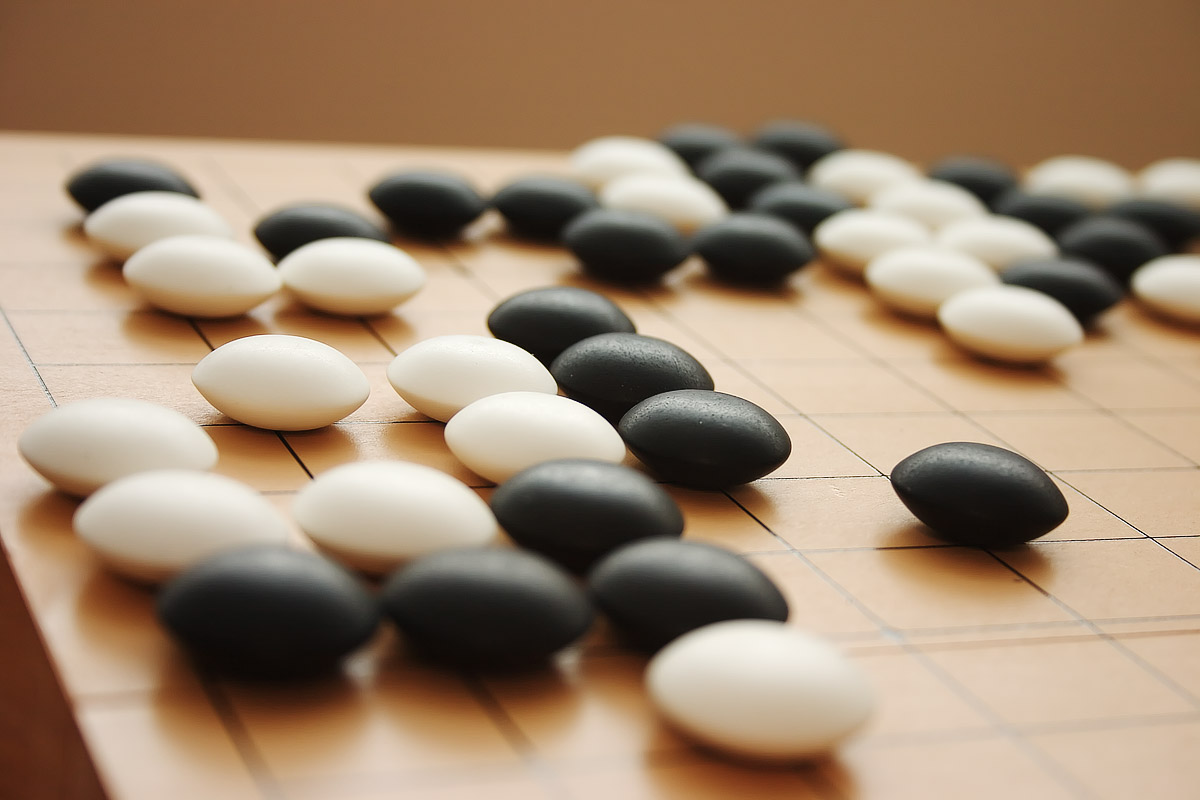
\includegraphics[height=\paperheight]{../img/Go_background.jpg}
    }
    \maketitle
  }

%%%%%%%%%%%%%%%%%%%%%%%%%%%%%%%%%%%%%%%%%%%%%%%%%%%%%%%%%%%%%%%%%%%%%%%%%%%%%%%%

  \section{Why AI?}

  \begin{frame}{Applications of AI}
    \begin{itemize}[<+- | alert@+>]
      \item spam filters
      \item recommender systems (Netflix, YouTube)
      \item predictive text (Swiftkey)
      \item audio recognition (Shazam, SoundHound)
      \item music generation (\cite{DeepHear})
      \item self-driving cars
    \end{itemize}
    \pause

    and...
  \end{frame}

  {
    \setbeamertemplate{frame footer}{\cite{Corrado15}}
    \begin{frame}{Auto Reply Feature of~Google Inbox}
      \begin{center}
        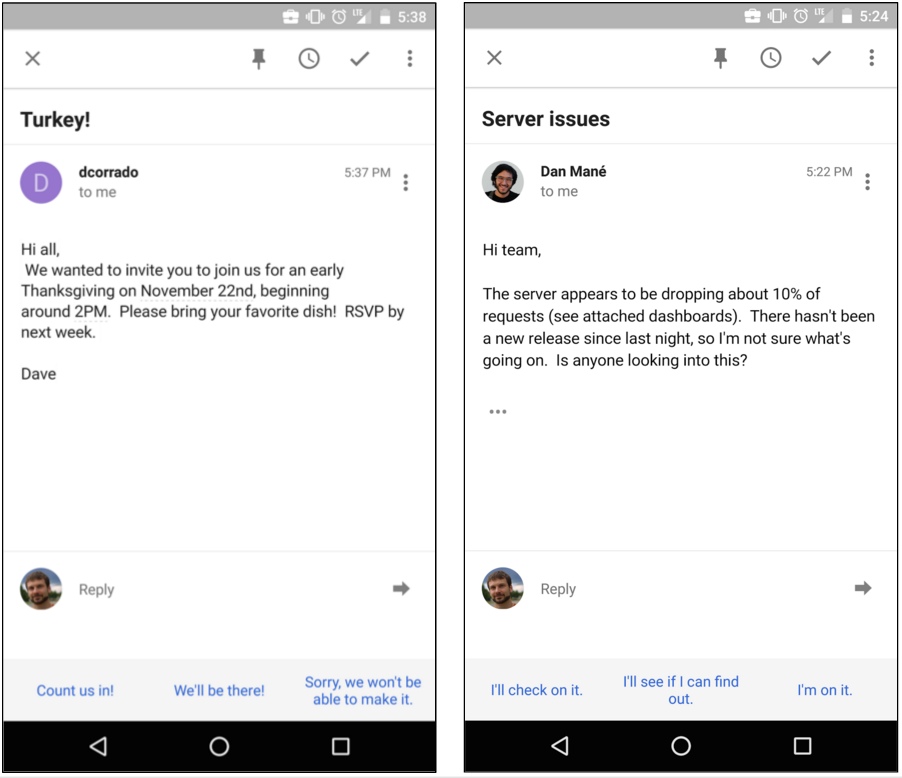
\includegraphics[height=.85\textheight]{../img/Inbox_auto_reply.png}
      \end{center}
    \end{frame}
  }

  {
    \setbeamertemplate{frame footer}{[1] \cite{GatysEB15a} [2] \cite{LiW16}}
    \begin{frame}{Artistic-style Painting}
      \begin{center}
        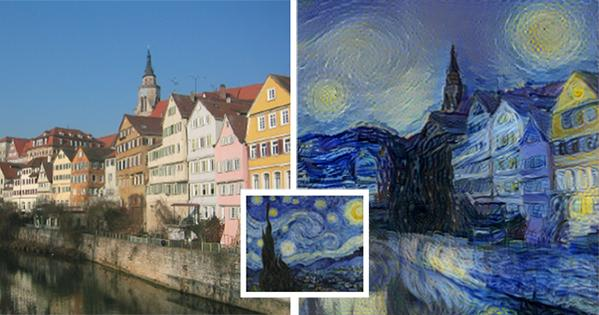
\includegraphics[height=.4\textheight]{../img/art_Van_Gogh.jpg}
        \pause

        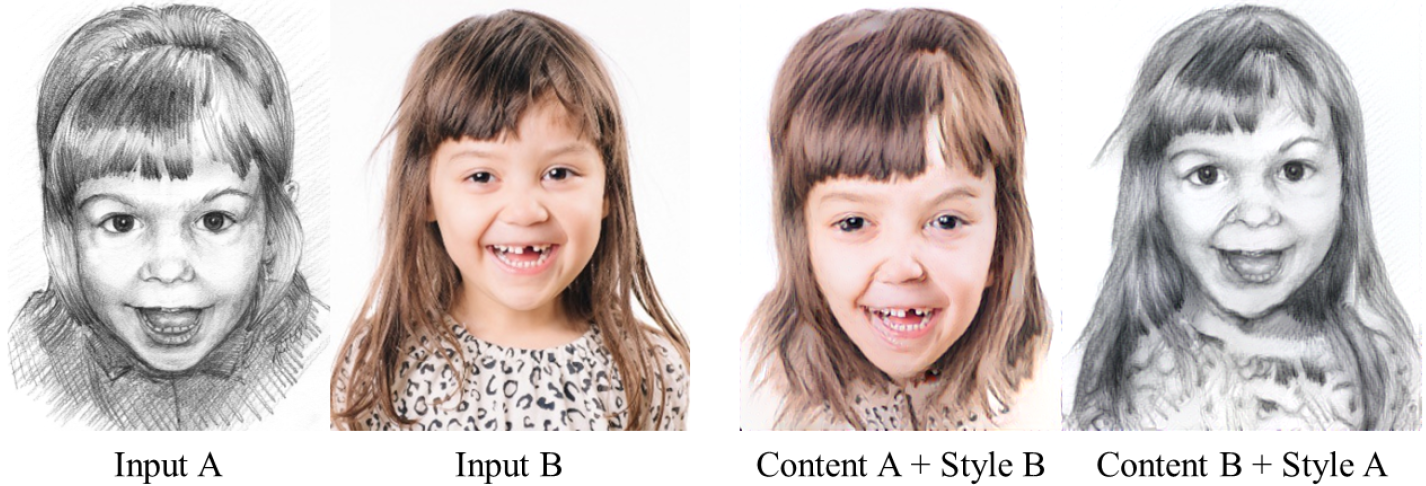
\includegraphics[height=.44\textheight]{../img/art_girl.png}
      \end{center}
    \end{frame}
  }

  {
    \setbeamertemplate{frame footer}{\cite{Karpathy15}}
    \begin{frame}{Baby Names Generated Character by Character}
      \begin{itemize}[<+- | alert@+>]
        \item Baby Killiel Saddie Char Ahbort With
        \item Rudi Levette Berice Lussa Hany Mareanne Chrestina Carissy
        \item Marylen Hammine Janye Marlise Jacacrie Hendred Romand Charienna Nenotto Ette Dorane Wallen Marly Darine Salina Elvyn Ersia Maralena Minoria Ellia Charmin Antley Nerille Chelon Walmor Evena Jeryly Stachon Charisa Allisa Anatha Cathanie Geetra Alexie Jerin Cassen Herbett Cossie Velen Daurenge Robester Shermond Terisa Licia Roselen Ferine Jayn Lusine Charyanne Sales Sanny Resa Wallon Martine Merus Jelen Candica Wallin Tel Rachene Tarine Ozila Ketia Shanne Arnande Karella Roselina Alessia Chasty Deland Berther Geamar Jackein Mellisand Sagdy Nenc Lessie Rasemy Guen
      \end{itemize}
    \end{frame}

    \begin{frame}{C code Generated Character by Character}
      \begin{center}
        \vskip -1.1ex
        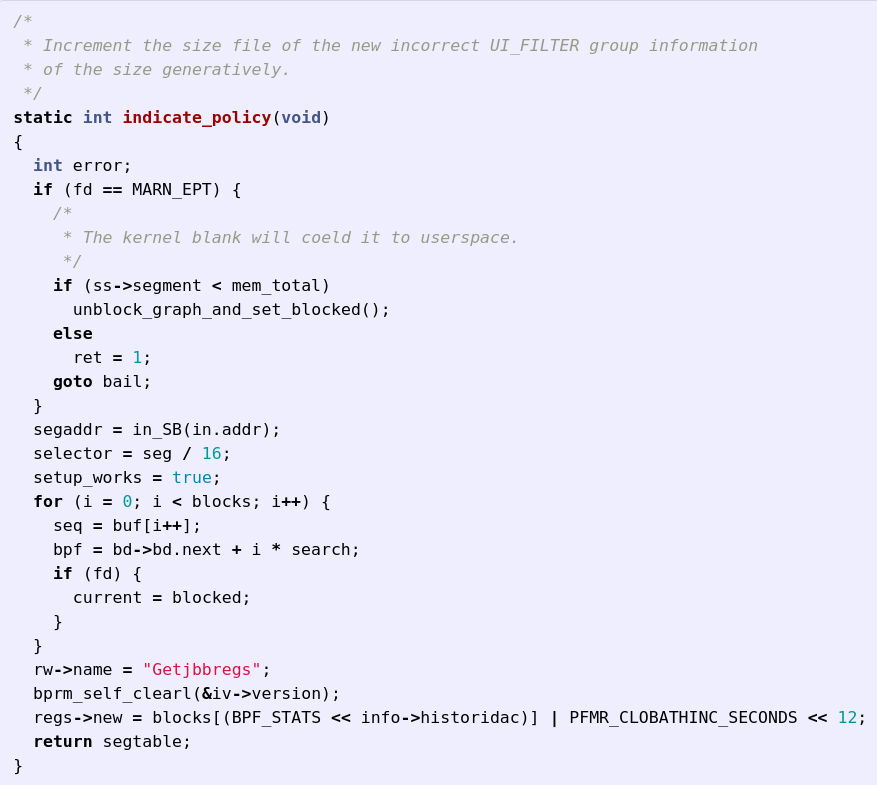
\includegraphics[height=.9\textheight, keepaspectratio]{../img/generating_c.png}
      \end{center}
    \end{frame}

    \begin{frame}{Algebraic Geometry Generated Character by Character}
      \begin{center}
        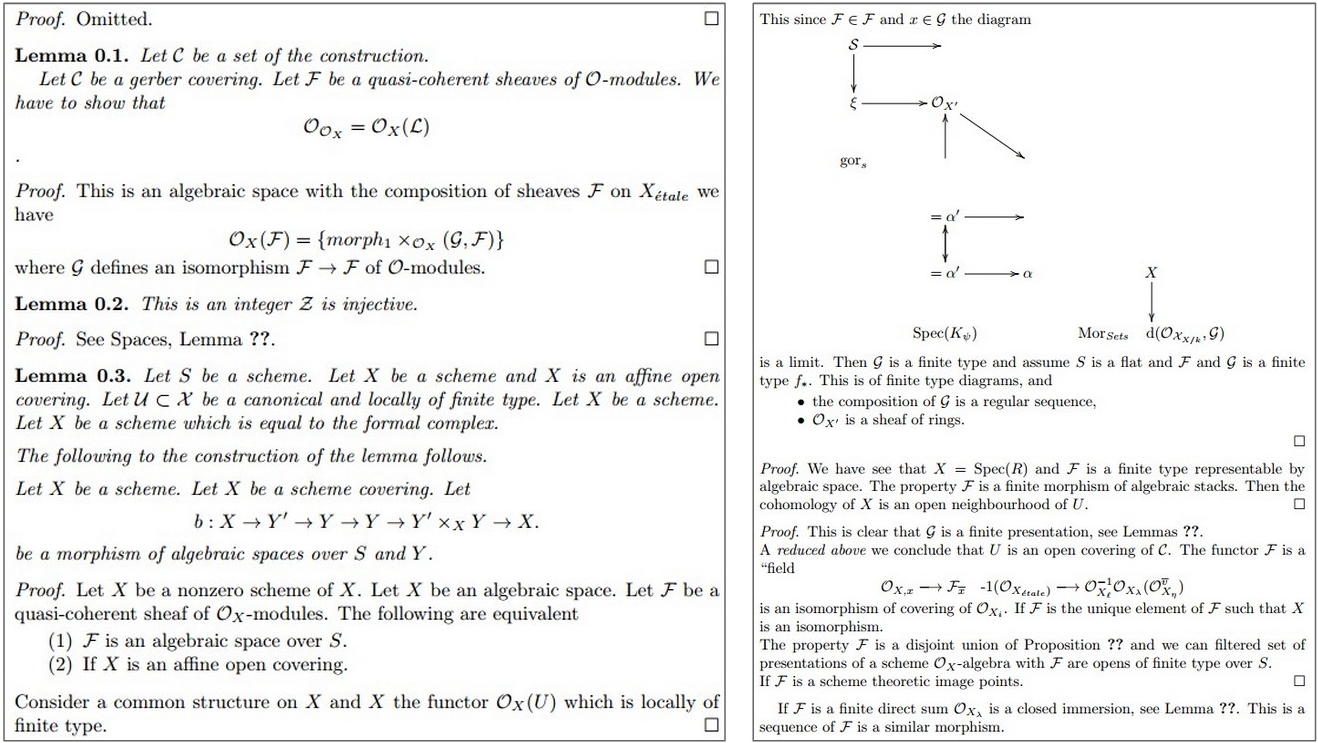
\includegraphics[width=\textwidth, height=\textheight, keepaspectratio]{../img/generating_latex.png}
      \end{center}
    \end{frame}
  }

  {
    \setbeamertemplate{frame footer}{\cite{DeepDrumpf}}
    \begin{frame}{DeepDrumpf}
      \url{https://twitter.com/deepdrumpf}
      \pause
      = a~Twitter bot that has learned the~language of~Donald Trump from his speeches 
      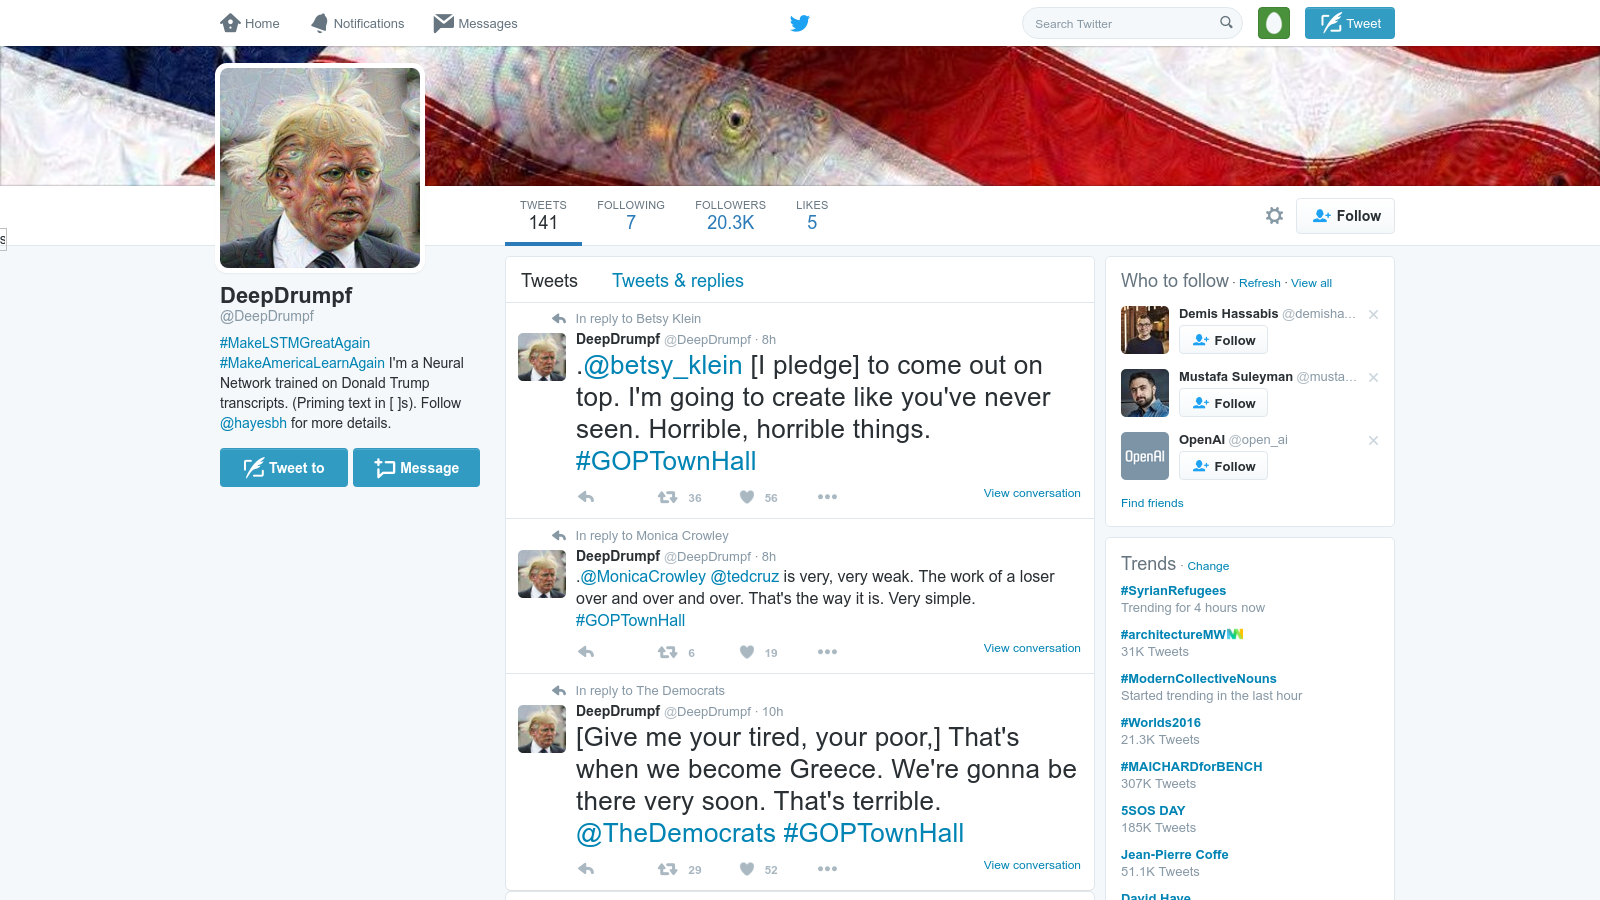
\includegraphics[width=\textwidth]{../img/DeepDrumpf.png}
    \end{frame}
  }

  {
    \setbeamertemplate{frame footer}{\cite{Mnih2015human}}
    \begin{frame}{Atari Player by Google DeepMind}
      \begin{center}
        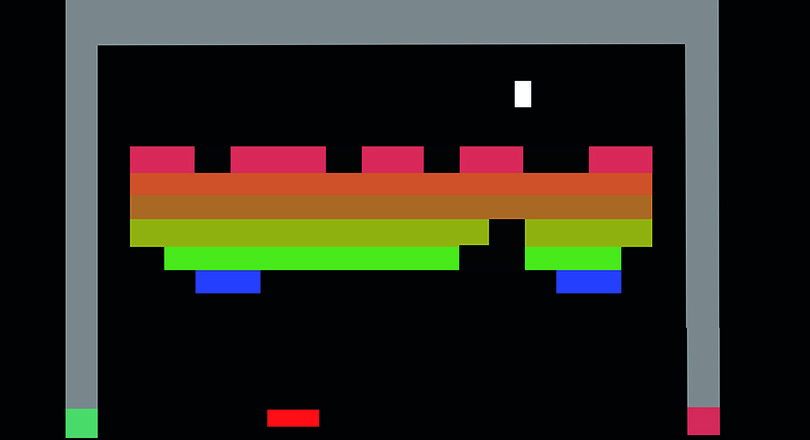
\includegraphics[width=\textwidth, height=\textheight, keepaspectratio]{../img/atari_breakout.jpg}

        \url{https://youtu.be/0X-NdPtFKq0?t=16m57s}
      \end{center}
    \end{frame}
  }

%%%%%%%%%%%%%%%%%%%%%%%%%%%%%%%%%%%%%%%%%%%%%%%%%%%%%%%%%%%%%%%%%%%%%%%%%%%%%%%%

  \section{Basics of Machine learning}

  \begin{frame}{Supervised versus Unsupervised Learning}
    Supervised learning
    \begin{itemize}[<+- | alert@+>]
      \item \todo
      \item \todo
    \end{itemize}
    \pause

    Unsupervised learning:
    \begin{itemize}[<+- | alert@+>]
      \item \todo
      \item \todo
    \end{itemize}
  \end{frame}

  \begin{frame}{Supervised Learning}
    Phases:
    \pause
    \begin{enumerate}[<+- | alert@+>]
      \item data collection: Google Search, Facebook ``Likes'', Siri, Netflix, YouTube views, LHC collisions...
      \item training on~\textbf{training set}
      \item testing on~\textbf{testing set}
      \item final deployment
    \end{enumerate}
    \pause
  \end{frame}

  \begin{frame}{Regression}
    \todo
  \end{frame}

  \begin{frame}{Classification}
    \todo
  \end{frame}

  {
    \setbeamertemplate{frame footer}{\url{https://www.researchgate.net/post/How_to_Avoid_Overfitting}}
    \begin{frame}{Underfitting and Overfitting}
      \begin{center}
        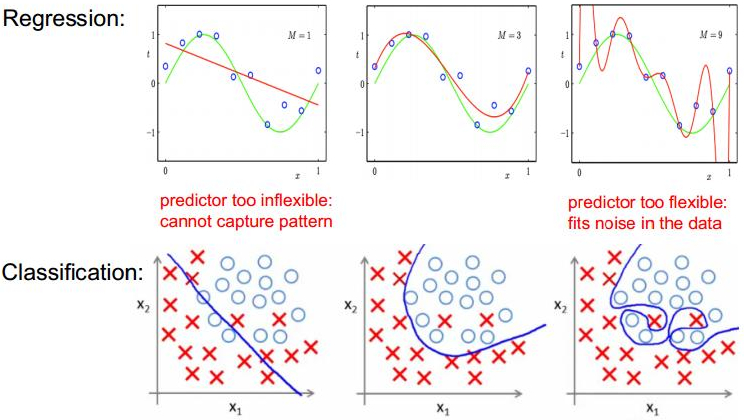
\includegraphics[width=.75\textwidth]{../img/underfitting_and_overfitting.jpg}
        \pause

        Beware of~overfitting!
      \end{center}
    \end{frame}
  }

  {
    \setbeamertemplate{frame footer}{\url{https://youtu.be/0X-NdPtFKq0?t=16m57s}}
    \begin{frame}{Reinforcement Learning}
      \begin{center}
        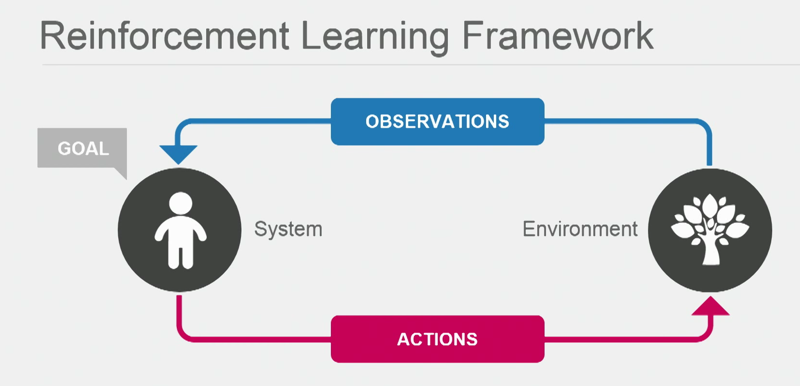
\includegraphics[width=\textwidth]{../img/RL_framework.png}
      \end{center}
      \pause
      
      Specially: games of \textbf{self-play}
    \end{frame}
  }

%%%%%%%%%%%%%%%%%%%%%%%%%%%%%%%%%%%%%%%%%%%%%%%%%%%%%%%%%%%%%%%%%%%%%%%%%%%%%%%%

  \section{Monte Carlo Tree Search}
  {
    \setbeamertemplate{frame footer}{\cite{Silver2016mastering}}
    \begin{frame}{Tree Search}
      Optimal value~$v^*(s)$ determines the~outcome of~the game:
      \pause
      \begin{itemize}[<+- | alert@+>]
          \tiny
        \item from every board position or state $s$
        \item under perfect play by~all players.
      \end{itemize}
      \pause

      It is computed by~\textbf{recursively traversing a~search tree} containing approximately $b^d$ possible sequences of moves, where
      \pause
      \begin{itemize}[<+- | alert@+>]
          \tiny
        \item $b$ is the game’s breadth (number of legal moves per position)
        \item $d$ is its depth (game length)
      \end{itemize}
    \end{frame}

    \begin{frame}{Game-tree of Go}
      \todo
    \end{frame}
  }

%%%%%%%%%%%%%%%%%%%%%%%%%%%%%%%%%%%%%%%%%%%%%%%%%%%%%%%%%%%%%%%%%%%%%%%%%%%%%%%%

  \section{Neural networks}
  \begin{frame}{Neural Network}
    \todo
  \end{frame}

  \begin{frame}{Deep Neural Network}
    \todo
  \end{frame}

  \begin{frame}{Convolutional Neural Network}
    \todo
  \end{frame}

%%%%%%%%%%%%%%%%%%%%%%%%%%%%%%%%%%%%%%%%%%%%%%%%%%%%%%%%%%%%%%%%%%%%%%%%%%%%%%%%

  \section{Rules of Go}
  \begin{frame}{Rules of Go}
    \emph{Black} versus \emph{White}.
    Black starts the game.

    \pause
    Two rules:
    \begin{description}
      \item [the rule of liberty] \todo
      \item [the ``ko'' rule] \todo
    \end{description}

    \pause
    \emph{Handicap} for difference in rank:
    Black can place 2 or more stones in advance (compensation for White's greater strength).
  \end{frame}

  \begin{frame}{Ranks}
    \todo
  \end{frame}

%%%%%%%%%%%%%%%%%%%%%%%%%%%%%%%%%%%%%%%%%%%%%%%%%%%%%%%%%%%%%%%%%%%%%%%%%%%%%%%%

  \section{AlphaGo: Inside Out}
  {
    \setbeamertemplate{frame footer}{\cite{Silver2016mastering}}
    \begin{frame}{Training the (Deep Convolutional) Neural Networks}
      \begin{center}
        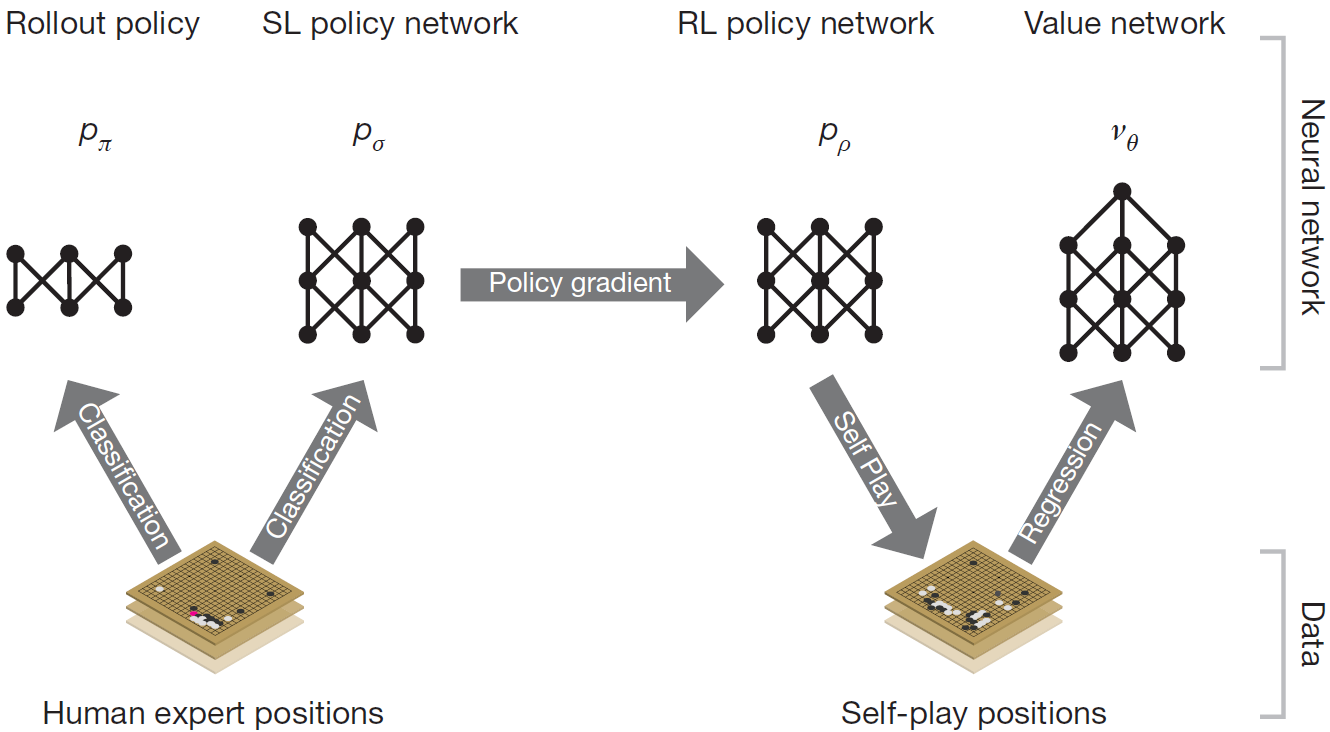
\includegraphics[width=\textwidth]{../img/neural_nets_pipeline.png}
      \end{center}
    \end{frame}

    \begin{frame}{Policy and Value Networks}
      \begin{center}
        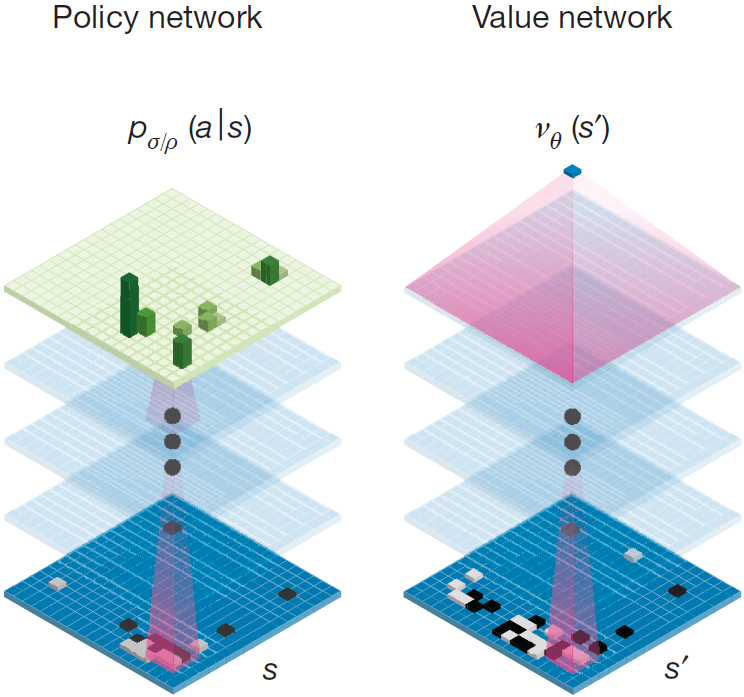
\includegraphics[height=.85\textheight]{../img/policy_and_value_network.png}
      \end{center}
    \end{frame}

    \begin{frame}{Rollout Policy}
      \todo
    \end{frame}

    \begin{frame}{SL Policy Networks (1/2)}
      \todo
    \end{frame}

    \begin{frame}{SL Policy Networks (2/2)}
      \begin{center}
        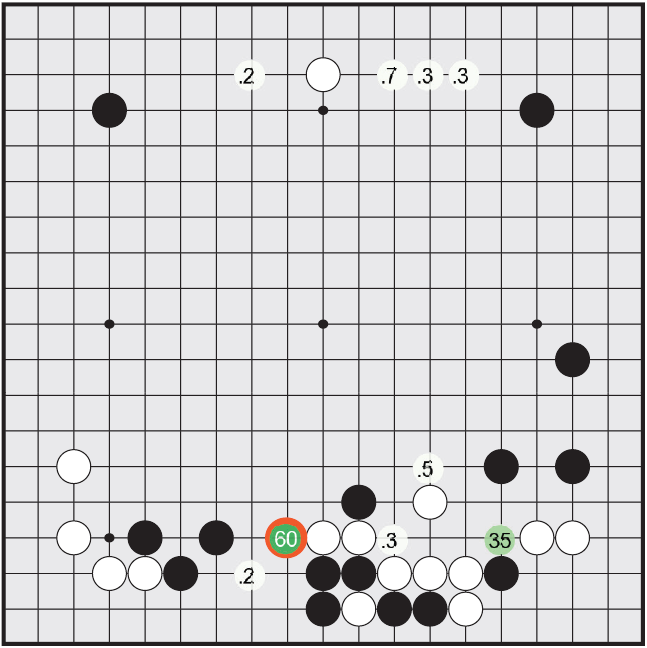
\includegraphics[height=.65\textheight]{../img/eval_SL_policy_network.png}
      \end{center}
      \vskip -1ex
      move probabilities taken directly from the SL policy network $p_\sigma$ (reported as a~percentage if above $0.1\%$).
    \end{frame}

    \begin{frame}{RL Policy Networks}
      \todo
    \end{frame}

    \begin{frame}{Value Network}
      \todo
    \end{frame}

    \begin{frame}{Selection of~Moves by the Value Network}
      \begin{center}
        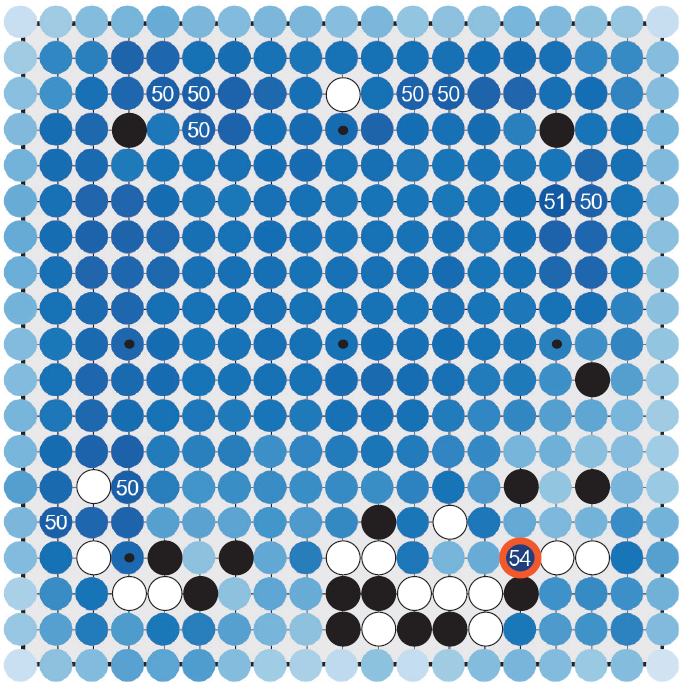
\includegraphics[height=.75\textheight]{../img/move_selection_by_value_network.png}
      \end{center}
      \vskip -1ex
      evaluation of~all successors $s'$ of~the root position~$s$, using~$v_\theta(s′)$
    \end{frame}

    \begin{frame}{ELO Ratings for~Various Combinations of~Networks}
      \begin{center}
        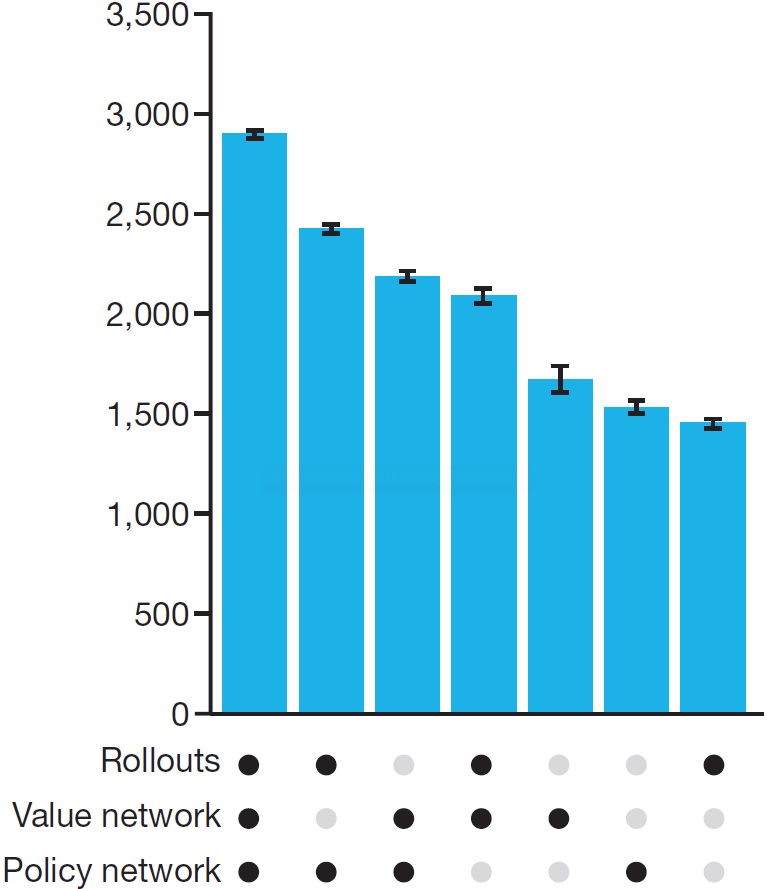
\includegraphics[height=.85\textheight]{../img/ELO_ratings_various_combinations_of_ANNs.png}
      \end{center}
    \end{frame}

    \begin{frame}{MCTS with Neural Networks (1/4)}
      \begin{center}
        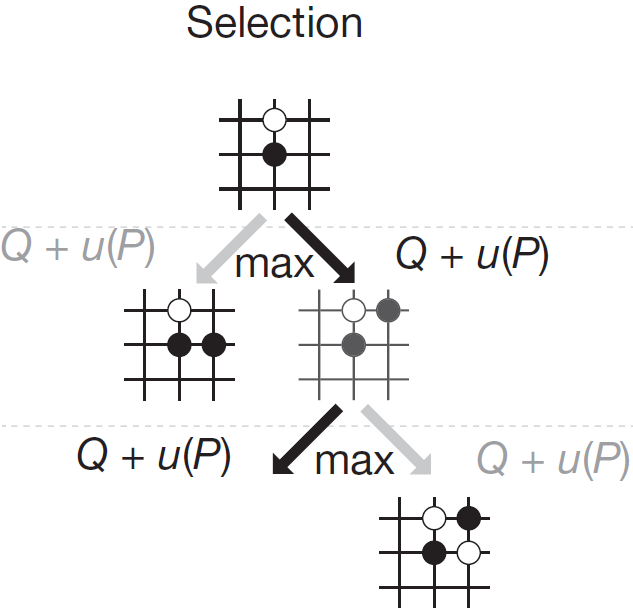
\includegraphics[height=.85\textheight]{../img/MCTS_selection.png}
      \end{center}
    \end{frame}

    \begin{frame}{MCTS with Neural Networks (2/4)}
      \begin{center}
        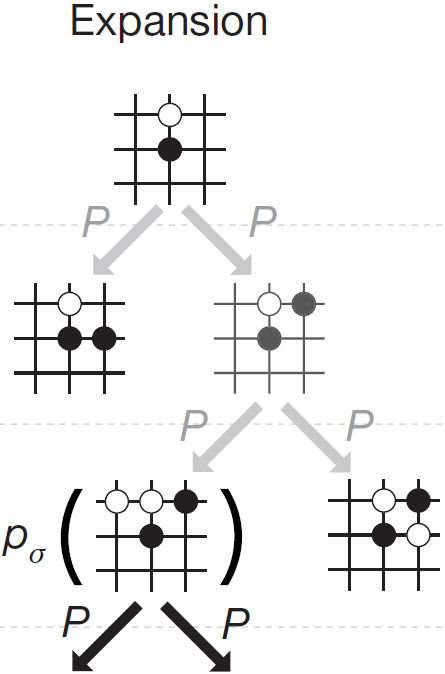
\includegraphics[height=.85\textheight]{../img/MCTS_expansion.png}
      \end{center}
    \end{frame}

    \begin{frame}{MCTS with Neural Networks (3/4)}
      \begin{center}
        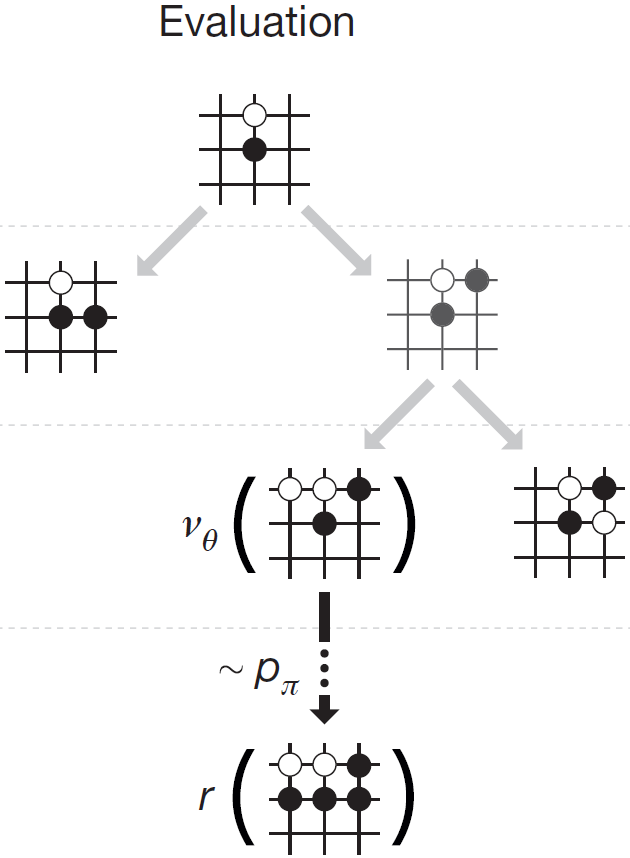
\includegraphics[height=.85\textheight]{../img/MCTS_evaluation.png}
      \end{center}
    \end{frame}

    \begin{frame}{MCTS with Neural Networks (4/4)}
      \begin{center}
        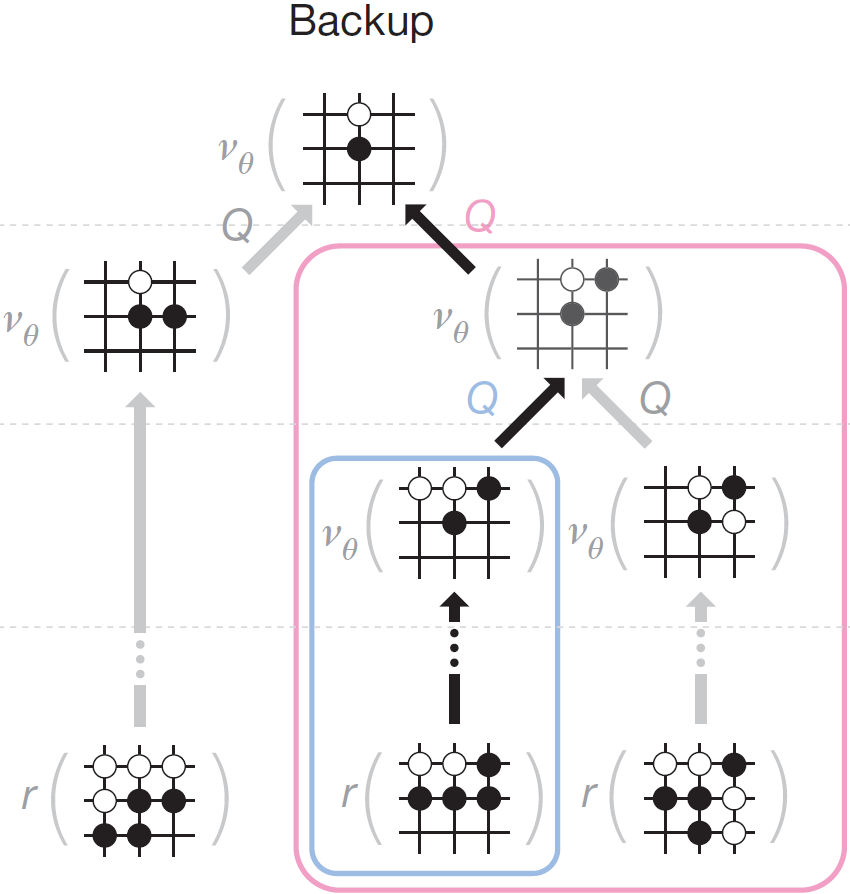
\includegraphics[height=.85\textheight]{../img/MCTS_backup.png}
      \end{center}
    \end{frame}

    \begin{frame}{Tree Evaluation from Value Network}
      \begin{center}
        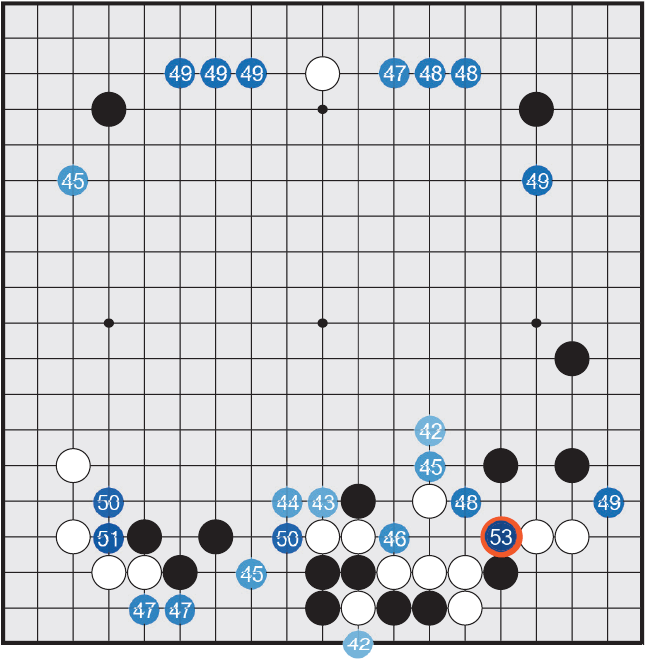
\includegraphics[height=.65\textheight]{../img/tree_eval_from_value_network.png}
      \end{center}
      \vskip -1ex
      action values~$Q(s, a)$ for~each tree-edge~$(s, a)$ from root position~$s$ (averaged over value network evaluations only)
    \end{frame}

    \begin{frame}{Tree Evaluation from Rollouts}
      \begin{center}
        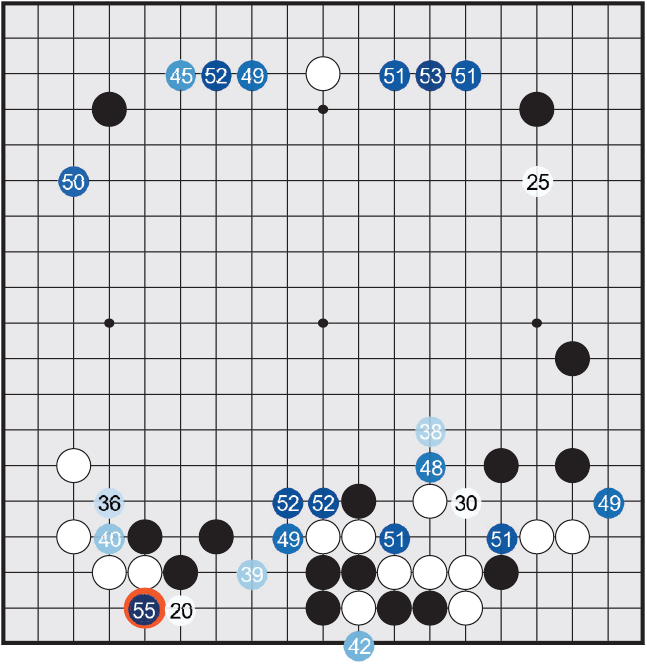
\includegraphics[height=.65\textheight]{../img/tree_eval_from_rollouts.png}
      \end{center}
      \vskip -1ex
      action values $Q(s, a)$, averaged over rollout evaluations only
      \vskip 1.45em
    \end{frame}

    \begin{frame}{Percentage of~Simulations}
      \begin{center}
        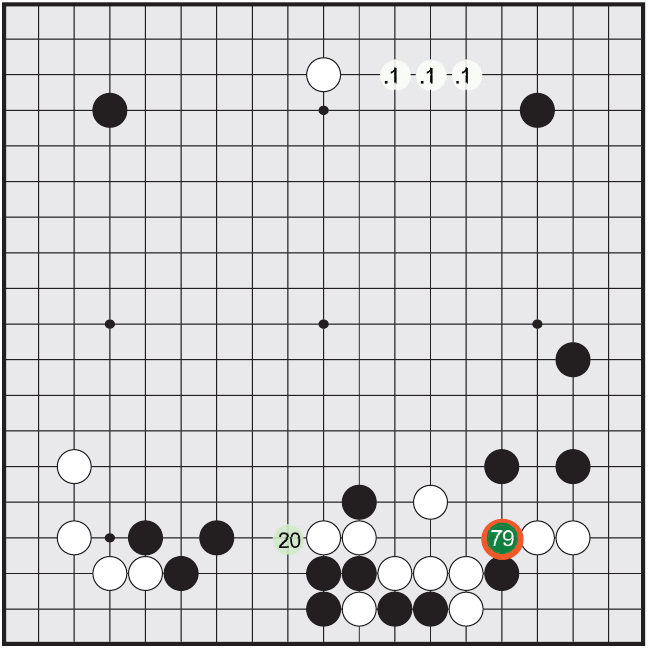
\includegraphics[height=.65\textheight]{../img/percentage_of_simulations.png}
      \end{center}
      \vskip -1ex
      percentage frequency with which actions were selected from the root during simulations
      \vskip 1.45em
    \end{frame}

    \begin{frame}{Principal Variation (Path with Maximum Visit Count)}
      \begin{center}
        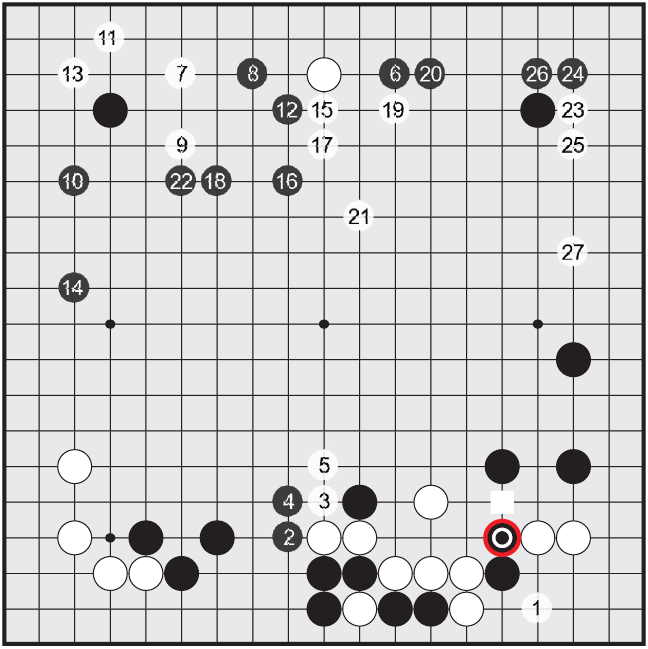
\includegraphics[height=.65\textheight]{../img/principal_variation.png}
      \end{center}
      \vskip -1ex

      The moves are presented in a numbered sequence.
      \pause
      \vskip -1ex
      \begin{tiny}
        \begin{itemize}[<+- | alert@+>]
          \item AlphaGo selected the move indicated by the red circle;
          \item Fan Hui responded with the move indicated by the white square;
          \item in his post-game commentary, he preferred the move (labelled 1) predicted by AlphaGo.
        \end{itemize}
      \end{tiny}
      \vskip 1.45em
    \end{frame}

    \begin{frame}{Scalability}
      \todo
    \end{frame}

    \begin{frame}{ELO Ratings for~Various Combinations of~Threads}
      \begin{center}
        \vskip -1ex
        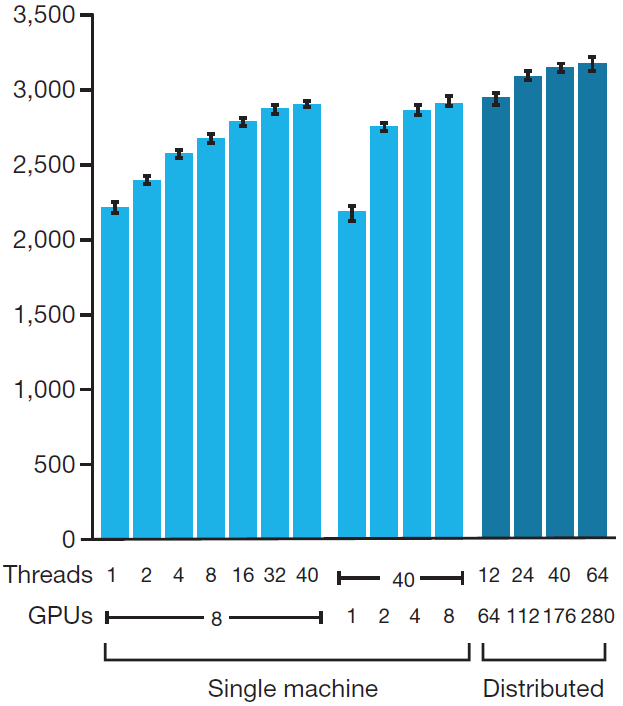
\includegraphics[height=.9\textheight]{../img/ELO_ratings_various_combinations_of_threads.png}
      \end{center}
    \end{frame}
  }

%%%%%%%%%%%%%%%%%%%%%%%%%%%%%%%%%%%%%%%%%%%%%%%%%%%%%%%%%%%%%%%%%%%%%%%%%%%%%%%%

  \section{Results: the strength of AlphaGo}

  {
    \setbeamertemplate{frame footer}{\cite{Silver2016mastering}}
    \begin{frame}{Tournament with Other Go Programs}
      \begin{center}
        \vskip -1ex
        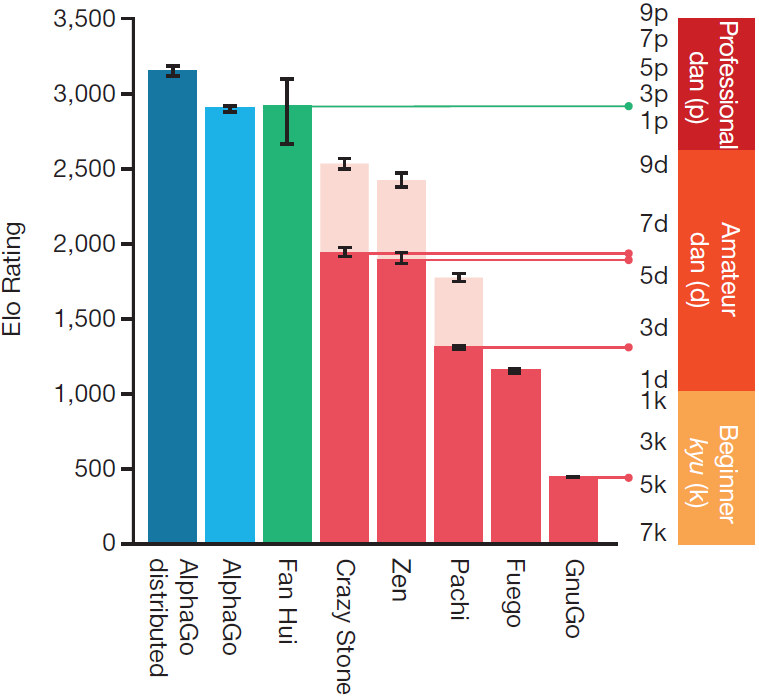
\includegraphics[height=.95\textheight]{../img/results_of_tournament.png}
      \end{center}
    \end{frame}

    \begin{frame}{AlphaGo versus Fan Hui}
      \todo
    \end{frame}

    \begin{frame}{AlphaGo versus Lee Sedol}
      \todo
    \end{frame}
  }

%%%%%%%%%%%%%%%%%%%%%%%%%%%%%%%%%%%%%%%%%%%%%%%%%%%%%%%%%%%%%%%%%%%%%%%%%%%%%%%%

  \section{Conclusion}

  \begin{frame}{Discussion}
    \todo
  \end{frame}

  \begin{frame}[standout]
    \begin{center}
      Thank you!
      \pause

      Questions?
    \end{center}
  \end{frame}

%%%%%%%%%%%%%%%%%%%%%%%%%%%%%%%%%%%%%%%%%%%%%%%%%%%%%%%%%%%%%%%%%%%%%%%%%%%%%%%%

  \appendix

  \begin{frame}[standout]
    Backup slides
  \end{frame}

  \begin{frame}{Further Reading}
    AI:
    \begin{itemize}
      \item \textbf{Singularity} \url{http://waitbutwhy.com/2015/01/artificial-intelligence-revolution-1.html} + Part 2
    \end{itemize}

    \todo
  \end{frame}

  \begin{frame}[allowframebreaks]{References}
    \tiny
    \printbibliography[heading=none]
  \end{frame}

\end{document}
